\chapter{Che cos'è la scienza cognitiva}
Con il termine ``scienze cognitive'' si definisce l'insieme di discipline che hanno come oggetto di studio la cognizione di un sistema pensante, sia esso naturale o artificiale. Esse comprendono diverse discipline che pur operando in campi differenti coniugano i risultati delle loro ricerche al fine comune di chiarire il funzionamento della mente.

Esse sono la neurofisiologia, la neuroscienza cognitiva, la psicologia cognitiva, l'intelligenza artificiale (AI), la inguistica cognitiva e la filosofia della mente, ma si vanno spesso ad esplorare territori di confine come l'antropologia, la genetica, l'etologia, l'economia (si pensi alla teoria dei giochi) e persino l'arte. Le principali di queste dottrine sono riunite nel cosiddetto \emph{esagono cognitivo}, che rappresenta la stretta interdisciplinarità di queste materie.

\begin{figure}[hbt]
  \centering
  \includegraphics[width=0.8\textwidth]{img/esagonocognitivo.jpg}
  \caption{Esagono cognitivo}
\end{figure}

Prima di addentrarsi nell'ambito della scienza cognitiva è bene chiarire la distinzione tra \emph{congizione}, \emph{cognitivismo} e \emph{psicologia cognitiva}.

La \emph{cognizione}\index{cognizione} è definita come l'insieme dei processi mentali appartenenti a due grandi categorie: i comportamenti cognitivi, che riguardano come conosciamo il mondo, e affettivi, che riguardano il modo in cui capiamo il mondo attraverso sentimenti ed emozioni. Tali descrizioni fanno già di per sé identificare come "cognitivi" processi quali la memoria, l'associazione, la formazione dei concetti, la pattern recognition, il linguaggio, l'attenzione, la percezione, l'azione, il problem solving e le immagini mentali.

Il concetto di cognizione è strettamente collegato ai concetti astratti di mente, ragionamento, percezione, intelligenza, apprendimento e molti altri ancora che descrivono le capacità della mente umana e le proprietà caratteristiche di intelligenza sintetica e dei gruppi collettivi che mostrano comportamento emergente.

In psicologia ed in intelligenza artificiale, il concetto di cognizione si utilizza parlando delle funzioni mentali, dei processi mentali, e degli stati di entità intelligenti (esseri umani, organizzazioni umane, robot altamente autonomi), in particolare quando si ha lo studio di processi come la comprensione, l'inferenza, la capacità di prendere decisioni e l'apprendimento.

Il \emph{cognitivismo}\index{cognitivismo}, invece, è la scuola di pensiero teorica derivata dall'approccio cognitivo, ed il complesso di metodi utilizzati per lo studio dei processi mentali.

La \emph{psicologia cognitiva}\index{psicologia cognitiva} è una branca della psicologia che ha come obiettivo lo studio dei processi mentali mediante i quali le informazioni vengono acquisite dal sistema cognitivo, elaborate, memorizzate e recuperate. Essa studia il funzionamento della mente come elemento intermedio tra il comportamento e l'attività cerebrale prettamente neurofisiologica. Il modello di funzionamento è assimilato metaforicamente a quello di un software che elabora informazioni provenienti dall'esterno (input), restituendo a sua volta informazioni (output) sotto forma di rappresentazione della conoscenza, organizzata in reti semantiche e cognitive.

\section{Filosofia}
Storicamente, due autorevoli discipline hanno interessato la formazione delle scienze cognitive: la filosofia e la psicologia.
La filosofia si occupa da millenni di diversi argomenti:
\begin{itemize}
  \item la natura della coscienza, e come questa sia acquistabile;
  \item il rapporto fra la mente e il corpo;
  \item in che modo emozioni e cognizioni interagiscono tra di loro.
\end{itemize}
Per spiegare il contributo della filosofia alla scienza cognitiva si deve fare innanzitutto riferimento al pensiero di René Descartes\index{Descartes, René}\footnote{René Descartes (La Haye en Touraine, 31 marzo 1596 – Stoccolma, 11 febbraio 1650) è stato un filosofo e matematico francese. È ritenuto fondatore della matematica e della filosofia moderna.} che, meglio di altri, rappresenta tale contributo.

\subsection{L'uomo macchina}
I due momenti essenziali nella storia delle scienze umane sono da un lato l'affermazione che il corpo dell'uomo è studiabile con mezzi empirici e non va trattato come sacro e, soprattutto, che la stessa assunzione possa essere estesa alla mente. René Descartes nel suo trattato \emph{De Hominem} (1662) è il primo ad effettuare un'analisi del corpo umano attraverso la ricostruzione ipotetica di una statua animata, costituita sul modello di una macchina. Sulla base dei risultati di dissezione e vivisezione su animali, Descartes giunge alla conclusione che le funzioni vitali dell'animale sono il risultato del calore e del movimento dei fluidi all'interno del corpo, estendendo poi questa ipotesi anche all'uomo.

Stanco dell'incertezza intrinseca nella filosofia, Descartes elabora un metodo basato sul dubbio sistematico, sintetizzato nell'aforisma \emph{cogito, ergo sum}. Siccome sulla capacità di dubitare si basa quella di pensare, allora egli basa la sua filosofia sulla mente, poiché in essa risiede la conoscenza. La prima conoscenza sicura è quella di sapere di star pensando, e quindi di esistere. Il \emph{cogito}, come capacità di autocoscienza appartiene solo agli uomini dotati di un corpo che funziona come una macchina: «...incomparabilmente meglio ordinata e ha in sé movimenti più meravigliosi di qualsiasi altra tra quelle che gli uomini possono inventare...»

All'interno della mente hanno un posto privilegiato le idee che si riferiscono a qualcosa di immutabile ed eterno, come l'aritmetica e la geometria, indipendenti dall'esistenza di entità analoghe nel mondo esterno, e tanto autoevidenti da poter essere considerate come generate dalla mente stessa.

Il corpo è invece assimilabile ad una macchina ed è sotto il controllo costante della mente, anche se non è ancora chiaro come tale controllo possa essere esercitato. Il corpo è pertanto composto da parti, che possono essere smontate, modificate, e sostituite senza che venga cambiato qualcosa di fondamentale. La mente, al contrario, non è scomponibile in parti separate, ma si tratta di un'unica complessa entità, dotata di caratteristiche particolari e irriducibili ad altro, fra cui spicca la capacità di trasmettere pensieri ad altre menti attraverso il linguaggio, che a sua volta non è riproducibile meccanicamente.

Julien Offray de La Mettrie\index{La Mettrie, Julien Offray de}\footnote{Julien Offray de La Mettrie (Saint-Malo, 25 dicembre 1709 – Potsdam, 11 novembre 1751) è stato un medico e filosofo francese, il primo scrittore materialista dell'illuminismo. È stato acclamato come fondatore delle scienze cognitive.} riprende il tema di Descartes sullo studio dell'uomo come macchina: a seguito della pubblicazione del libro \emph{L'homo machine} nel 1748, è costretto all'esilio per due volte; prima a Leida, dove riuscì a pubblicare il libro, che però viene bruciato dal boia nella pubblica piazza, ad ammonimento ai diffusori dell'ateismo, costringendolo ad un secondo esilio.

La Mettrie, nel suo trattato, pone alla base dell'uomo un'unica proprietà, il movimento, come essenziale per spiegare come l'uomo pensi, senta e agisca. Inoltre, il fatto che si possa dimostrare in modo evidente una correlazione tra stati psichici e corporei, permette di considerare gli eventi mentali come risultato delle funzioni cerebrali e non prodotto di un'anima immateriale.

Pochi anni dopo, le sue teorie vennero riprese apertamente dai \emph{méchaniciens}, un gruppo di studiosi che consideravano l'uomo come una macchina e lo studiavano come tale, che Diderot e D'Alembert definivano nell'Encyclopédie: «Si chiamano così quei medici moderni che, dopo la scoperta della circolazione del sangue e il diffondersi della filosofia di Descartes, hanno scosso il giogo dell'autorità e hanno adottato il metodo dei geometri nelle ricerche che hanno fatto su ciò che concerne l'economia animale [\dots] Il corpo animale, e di conseguenza il corpo umano, è quindi considerato come una vera e propria macchina.»

Nel frattempo l'inventore francese Jacques de Vaucanson\index{de Vaucanson, Jacques}\footnote{Jacques de Vaucanson (Grenoble, 24 febbraio 1709 – Parigi, 21 novembre 1782) è stato un inventore e artista francese, celebre per l'invenzione e costruzione di numerosi complessi automi.} comincia a costruire una serie di automi, tra cui un'anatra e un flautista, nei quali riproduce fedelmente con parti meccaniche ciò che era noto in anatomia e fisiologia. L'obiettivo più ambizioso è quello di costruire un essere umano e, anche se non verrà mai realizzato dallo scienziato, già il fatto che se ne parlasse come un progetto possibile fu un fatto straordinario.

La Rivoluzione francese sancisce in modo definitivo il principio per cui corpo e mente dell'uomo possono essere indagabili e non più sacri e inviolabili. Su queste basi nasce la moderna scienza dell'uomo, che è scoperta del vero e avanzamento della conoscenza umana.

\section{La nascita della scienza cognitiva}
\subsection{Meccanizzazione del calcolo}
La cibernetica prefigura la scienza cognitiva e l'intelligenza artificiale. Essa estende l'uso dei calcolatori affrontando temi come le reti neurali, la razionalizzazione del traffico, sistemi di controllo, ecc. Le sue origini risalgono anch'esse verso la fine del Settecento.

In quel periodo, infatti, il governo francese incaricò l'ingegnere Gaspard de Prony\index{de Prony, Gaspard}\footnote{Gaspard Riche barone di Prony (Chamelet, 22 luglio 1775 – Parigi, 29 luglio 1839) è stato un ingegnere, matematico e musicologo francese. Studioso dai vasti interessi, si occupò approfonditamente di una notevole gamma di problemi attinenti all'ingegneria e assai spesso a diverse altre discipline, meritandosi l'appellativo di "encyclopédiste".} di compiere l'incredibile opera di compilare le tavole logaritmiche e trigonometriche fino a $200000$. Prony, ispirandosi al lavoro di Adam Smith sulla suddivisione del lavoro, ebbe l'idea di dividere la computazione dei logaritmi su più uomini. In questo modo si rendeva possibile il lavoro che un solo cervello non sarebbe mai stato in grado di compiere, riducendo il livello di difficoltà creando piccoli compiti di operazioni semplici e ripetitive. Mediante precise regole di ricomposizione delle operazioni e dei loro risultati, si ottiene così il risultato finale della complessa operazione logaritmica di partenza.

\subsection{La macchina analitica}\index{macchina analitica}
Il passo successivo consiste nel concepire una macchina in grado di gestire informazioni complesse, che non limitino l'attività alla manipolazione di cifre. È Charles Babbage\index{Babbage, Charles}\footnote{Charles Babbage (Walworth, 26 dicembre 1791 – Londra, 18 ottobre 1871) è stato un matematico e filosofo britannico, scienziato proto-informatico che per primo ebbe l'idea di un calcolatore programmabile.}, con la sua \emph{macchina analitica} proposta nel 1833, a compiere tale passo. Egli contava di rendere le specifiche operazioni governate da un programma; cambiato il programma, la macchina avrebbe potuto eseguire compiti diversi. Creò così l'idea di macchina \emph{general purpose}, che purtroppo per mancanza di finanziamenti e di precisione della tecnologia manifatturiera, non vide mai la luce.

La struttura generale della macchina è molto simile al concetto odierno di calcolatore: è previsto un ``mulino per macinare dati'' (cpu) e un ``deposito per immagazzinarli'' (memoria).

\begin{figure}[hbt]
  \centering
  \includegraphics[width=0.6\textwidth]{img/AnalyticalMachine_Babbage_London.jpg}
  \caption{Modello di una parte dell'Analytical Engine di Babbage in mostra al Museo della scienza di Londra (credits: Bruno Barral)}
  \label{}
\end{figure}


Ada Lovelace\index{Lovelace, Ada}\footnote{Augusta Ada Byron, meglio nota come Ada Lovelace (Londra, 10 dicembre 1815 – Londra, 27 novembre 1852), è stata una matematica inglese, nota soprattutto per il suo lavoro alla macchina analitica ideata da Charles Babbage. Tra i suoi appunti sulla macchina di Babbage si rintraccia anche un algoritmo per generare i numeri di Bernoulli, considerato come il primo algoritmo espressamente inteso per essere elaborato da una macchina, tanto che Ada Lovelace è spesso ricordata come la prima programmatrice di computer al mondo.}, collaboratrice di Babbage e allieva di De Morgan, fu la prima a distinguere tra calcolatore e programma per calcolare, ovvero a creare la distinzione tra hardware e software, che resta valida tutt'oggi.

L'interesse del governo inglese per la macchina analitica era motivato dalla necessità di disporre di una macchina che potesse automatizzare il calcolo delle operazioni complesse, per rendere più sicura e corretta la navigazione della flotta inglese. Anche se tale macchina non fu mai realizzata, il denaro investito non fu considerato perso dal governo: fu comunque un passo avanti verso l'automazione del lavoro manuale.

\subsection{Le leggi del pensiero}\index{logica matematica}
Le basi della logica moderna furono gettate dal matematico George Boole\index{Boole, George}\footnote{George Boole (Lincoln, 2 novembre 1815 – Ballintemple, 8 dicembre 1864) è stato un matematico e logico britannico, ed è considerato il fondatore della logica matematica. La sua opera influenzò anche settori della filosofia.}, a Cambridge. I suoi obiettivi erano chiari: indagare le leggi delle operazioni della mente per mezzo delle quali si attua il ragionamento, dar loro espressione nel linguaggio simbolico e, in ultimo, ricavare indicazioni sulla natura e la costituzione della mente umana. Seguendo un metodo generale di derivazione si possono raggiungere conclusioni certamente vere, indipendentemente dai contenuti specifici del ragionamento. La verità logica si sposta dai significati, dalle interpretazioni date a simboli e connettivi, alle relazioni e regole astratte che vanno seguite.

Boole pensava che le regole che stanno alla base della logica fossero le stesse che governano il pensiero umano. Questo approccio, di cui egli fu il principale rappresentante, viene chiamato logica mentale. L'ipotesi fondamentale di tale approccio è che esiste una logica della mente che corrisponde a quella formale.

\section{La cibernetica}\index{Cibernetica}
La cibernetica (dal greco \emph{kibernetes}, pilota di una nave) viene fondata da Norbert Wiener\index{Wiener, Norbert}\footnote{Norbert Wiener (Columbia, 26 novembre 1894 – Stoccolma, 18 marzo 1964) è stato un matematico e statistico statunitense. Famoso per ricerche sul calcolo delle probabilità ma soprattutto per gli sviluppi dati, insieme al suo allievo Claude Shannon, alla teoria dell'informazione essendo riconosciuto come il padre della cibernetica moderna.} assieme al fisiologo Rosenblueth, l'ingegnere Bigelow e il logico Pitts, precorrendo informatica, intelligenza artificiale e scienza cognitiva.

La parola cibernetica fu reintrodotta\footnote{Nel greco di Platone è già attestata la parola kybernetikè, che dal significato originario di governare una nave acquista per metafora il senso del governare una città o uno Stato. Nel 1834 Ampère riprende il termine greco nella sua ampia classificazione delle scienze, francesizzando la parola nell'accezione politica già attestata in Platone.} da Wiener nell'estate del 1947 anglicizzandola in cybernetics, nell'atto di dare il titolo al libro che uscirà l'anno dopo: \emph{Cybernetics or Control and Communication in the Animal and the Machine}; quest'atto coincise anche con il battesimo di una nuova scienza a cui Wiener pensava da tempo, fondata appunto sullo studio di animali e macchine dal punto di vista della teoria dei controlli automatici e delle telecomunicazioni. Norbert Wiener scrive in questo libro di aver voluto, tra le altre cose, rendere omaggio a James Clerk Maxwell, autore di \emph{On Governors}, una delle prime fondamentali descrizioni matematiche del comportamento dei cosiddetti regolatori centrifughi di velocità, dove vengono individuate le condizioni di un loro comportamento stabile. Il primo di tali regolatori era stato introdotto nel 1789 da James Watt per controllare le variazioni di carico delle sue macchine a vapore. D'altro canto la cibernetica per Wiener non è soltanto controllo ma anche comunicazione; anzi quest'ultima ha la priorità per la comprensione degli stessi controlli automatici.

Nel 1944 Wiener organizza, assieme a von Neumann, il primo convegno di cibernetica, dove emerse che campi diversi come matematica, logica, fisiologia e ingegneria elettronica ruotavano appunto attorno al concetto di \emph{feedback}, o retroazione\index{feedback}. Ogni volta in cui si deve modificare un sistema secondo un modello, si utilizza la differenza tra le rilevazioni del sistema e il modello in un determinato istante, come segnale per determinare una correzione del sistema stesso. L'esempio classico è quello del termostato, che corregge l'apporto di calore a seconda della rilevazione della temperatura esterna.

In generale, si distingue in due tipi di feedback: quello \emph{negativo} (come nell'esempio del termostato), nel quale si tende a stabilizzare la situazione attorno al punto desiderato, opponendosi al corso naturale del sistema, e quello \emph{positivo},  nel quali invece si tende ad ampliare le oscillazioni del sistema ed utilizza un controllo esterno per interrompere il circuito una volta raggiunto uno stato limite.

In neurofisiologia gli esempi di feedback negativo, basati su un comportamento teso a minimizzare le differenze fra stato iniziale e stato desiderato, sono molteplici. Lo scopo di tali processi retroattivi è quello di garantire l'\emph{omeòstasi}\index{omeostasi}, ovvero uno stato in cui il sistema è in condizioni ottimali.

Nell'ottica della cibernetica, l'uomo sopravvive grazie ad un numero di circuiti retroattivi fisiologici e neurali che garantiscono che venga appunto mantenuta l'omeostasi. Grazie a questo concetto di feedback è possibile parlare di \emph{scopo} non solo per gli esseri viventi, ma anche per le macchine, a patto che queste siano dotate della possibilità di controllare il comportamento durante l'esecuzione. La differenza essenziale è che il fine della macchina è imposto dall'esterno, attraverso i vincoli fisici e la loro regolazione.

In seguito, il gruppo di studiosi di cibernetica si allargò, includendo psicologi, antropologi e sociologi. Nell'opera \emph{Cybernetics} (1948), Weiner spiega come la cibernetica nasceva dalla consapevolezza che sia le macchine sia gli esseri viventi condividono gli stessi problemi riguardo la comunicazione e il controllo.

Nonostante il periodo bellico, i cibernetici furono antimilitaristi, mostrandosi attenti alle applicazioni delle loro ricerche, concentrandosi su quelle mediche, psicologiche e sociali.

L'intenzionalità\index{intenzionalità} delle macchine, di qualunque genere esse siano, è sempre \emph{come se}. Si comportano cioè come se avessero intenzionalità propria; un osservatore può descriverle come se fossero dotate di intenzionalità, ma resta sempre e solo una attribuzione esterna. L'intenzionalità effettiva è quella del programmatore, anche se i circuiti retroattivi mostrano un comportamento teleologico\footnote{che ha un fine, anche se il suo comportamento è inconsapevole o involontario}, in questo caso perché fornito dall'esterno. In particolare, gli automi cibernetici possiedono sensori preposti alla percezione delle variazioni ambientali, attuatori in grado di eseguire azioni e circuiti che trasmettono le informazioni tra le parti.

\subsection{La macchina di Turing}
Nel tentativo di analizzare i passi successivi secondo cui un essere umano esegue un calcolo, nel 1937 Alan Turing\index{Turing, Alan}\footnote{Alan Mathison Turing (Londra, 23 giugno 1912 – Wilmslow, 7 giugno 1954) è stato un matematico, logico e crittografo britannico, considerato uno dei padri dell'informatica e uno dei più grandi matematici del XX secolo.} propose l'idea di un automa astratto chiamato ``macchina di Turing''. Questa macchina manipola i dati contenuti su un nastro di lunghezza potenzialmente infinita secondo un insieme di regole precise. Di fatto, è un modello astratto per definire la calcolabilità e la complessità degli algoritmi.

\begin{figure}[hbt]
  \centering
  \includegraphics[width=0.5\textwidth]{img/turingMachine.png}
  \caption{La macchina di Turing}
\end{figure}	

La macchina può agire sopra un nastro che si presenta come una sequenza di caselle nelle quali possono essere registrati simboli di un ben determinato alfabeto finito (ad esempio quello dei calcolatori, il sistema binario composto da 0 e 1); essa è dotata di una testina di lettura e scrittura (I/O) con cui è in grado di effettuare operazioni di lettura e scrittura su una casella del nastro. La macchina evolve nel tempo e ad ogni istante si può trovare in uno stato interno ben determinato facente parte di un insieme finito di stati. Inizialmente sul nastro viene posta una stringa che rappresenta i dati che caratterizzano il problema che viene sottoposto alla macchina. La macchina è dotata anche di un repertorio finito di istruzioni che determinano la sua evoluzione in conseguenza dei dati iniziali. L'evoluzione si sviluppa per passi successivi che corrispondono a una sequenza discreta di istanti successivi. Le proprietà precedenti sono comuni a molte macchine formali (automa a stati finiti, automa a pila, ecc).

Ogni passo dell'evoluzione viene determinato dallo stato attuale $s$ nel quale la macchina si trova e dal carattere $c$ che la testina di I/O trova sulla casella del nastro su cui è posizionata e si concretizza nell'eventuale modifica del contenuto della casella, nell'eventuale spostamento della testina di una posizione verso destra o verso sinistra e nell'eventuale cambiamento dello stato. Quali azioni vengono effettuate ad ogni passo viene determinato dall'istruzione, che supponiamo unica, che ha come prime due componenti $s$ e $c$; le altre tre componenti dell'istruzione forniscono nell'ordine il nuovo stato, il nuovo carattere e una richiesta di spostamento verso sinistra, nullo o verso destra.

L'importanza della macchina di Turing è tale che oggi, per definire in modo formalmente preciso la nozione di algoritmo, si tende a ricondurlo alle elaborazioni effettuabili con macchine di Turing.

\section{La teoria dell'informazione}\index{teoria dell'informazione}
In termini di comunicazione, una giustificazione formale dell'equivalenza tra macchina e uomo fu elaborata da Claude Shannon\index{Shannon, Claude}\footnote{Claude Elwood Shannon (Petoskey, 30 aprile 1916 – Medford, 24 febbraio 2001) è stato un matematico e ingegnere statunitense, spesso definito il padre della teoria dell'informazione} e Warren Weaver con la teoria dell'informazione. Il primo obiettivo della teoria fu quello di misurare quantitativamente l'informazione, in rapporto alla quantità massima di informazione trasmessa attraverso un canale di comunicazione. La quantità di informazione si può definire come costante intrinseca del messaggio, indipendentemente da come esso sia codificato e dalla modalità di trasmissione e ricezione.

L'informazione è definita come variazione di uno stato e la più elementare è la variazione di un segnale da 0 a 1 e viceversa. Questa informazione è considerata unitaria e denominata ``bit'' (\emph{binary unit}). Un bit può essere usato per discriminare fra due alternative equiprobabili; per discriminare fra quattro alternative servono 2 bit, e via dicendo. Se chiamiamo $I$ l'informazione trasmessa, allora $I = \log (\text{numero di alternative})$. Questa formula indica che il contenuto informativo (autoinformazione) di un messaggio corrisponde al logaritmo in base 2 del numero di alternative possibili. Dato che la probabilità $p(m)$ di un messaggio è inversamente proporzionale al numero delle alternative possibili, abbiamo
\begin{equation}
	I = -\log_{2}{p(m)}.
\end{equation}

Questo corrisponde a dire che la quantità di informazione contenuta in un messaggio è misurata dal logaritmo negativo in base 2 della probabilità del messaggio stesso.

Non solo il valore informativo varia da messaggio a messaggio, ma anche all'interno dello stesso messaggio il valore di ciascun componente non è equivalente, perché è legato alla novità, ovvero a quanto il ricevente se lo aspetta (ad esempio, se tutti i giorni dico che c'è il sole, dopo un po' il contenuto informativo diventa nullo, se dico che nevica, c'è molta più informazione; le prime lettere di una parola sono più informative perché discriminano una parola da tutte le altre).

Questo approccio statistico è simile a quello della termodinamica statistica: entrambi hanno in comune il concetto di \emph{entropia}\index{entropia}, ovvero il contenuto medio di informazione. Per Shannon l'informazione contenuta in un messaggio è tanto maggiore quanto maggiore è l'indipendenza fra i vari elementi del messaggio (ad esempio,  un messaggio cifrato ha entropia massima, non ci sono correlazioni statistiche tra le parti del messaggio, ovvero tutti i simboli sono equiprobabili). Equivalentemente, l'entropia del sistema ricevente diminuisce alla ricezione di un messaggio informativo, perché questo diminuisce la sua incertezza rispetto al mondo.

Formalmente l'entropia $H$ si costruisce a partire dalla definizione di autoinformazione ed è definita come misura dell'incertezza associata ad una variabile aleatoria $X$.
\begin{equation}
H(X) = \mathbb{E}_{X} [I(x)] = -\sum_{x \in \mathbb{X}} p(x) \log p(x).	
\end{equation}

Come si può notare dalla figura \ref{fig:entropia}, l'incertezza è massima quando la probabilità del simbolo del messaggio è 0.5, mentre è minima quando l'evento è certo o nullo. È intuitivo pensare che se stiamo ricevendo dei bit su un canale, dato un simbolo trasmesso (ad esempio, 1), la probabilità di ricevere l'opposto (in questo caso, 0) sia del 50\%, e dunque l'incertezza è massima. Se siamo sicuri di ricevere lo stesso bit (o il suo opposto) allora l'incertezza è nulla (nel caso di valore opposto, basta invertire sempre il bit per ottenere il valore trasmesso).
\begin{figure}[hbt]
  \centering
  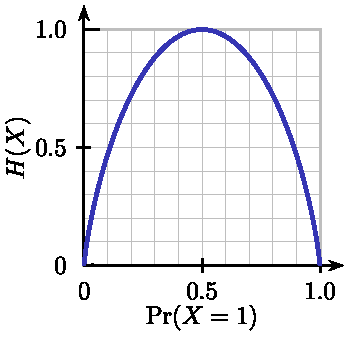
\includegraphics{img/Binary_entropy_plot}
  \caption{Entropia di una variabile di Bernoulli.}
  \label{fig:entropia}
\end{figure}

\subsection{Reti neurali}
Dapprima in modo indipendente dai lavori di Shannon sulla teoria dell’informazione e poi in piena sintonia con essa, McCulloch e Pitts svilupparono le ricerche cibernetiche in campo neurologico. Essi dimostrarono che qualunque funzione computabile può venire calcolata da una rete opportuna di neuroni ideali, elementi a soglia le cui proprietà possono essere attribuite ai neuroni reali. Il problema consiste nel trovare un principio generale di autorganizzazione della rete neurale, tale da permettere alla rete di risolvere alcuni problemi prototipo, come il riconoscimento delle forme. Affronteremo più in dettaglio l'argomento nella sezione \S \ref{reti-neurali} a pagina \pageref{reti-neurali}.
